\chapter{Design del sistema}

\section{Design Goals}
Il design di un sistema software deve essere svolto a valle di un'attenta 
analisi degli obiettivi di design, tradeoffs nell'ambito delle qualitá del 
software che rendano il software il piú adatto possibile per le sue ragioni 
di essere.

Il design del sistema deve essere costruito a partire dai requisiti non funzionali
descritti nel capitolo precedente.

\section{Design di alto livello}
Il sistema è suddiviso in due macro-componenti distribuite, comunicanti tramite 
rete:
\begin{list}{$\cdot$}{}
    \item Front-end. Il software che fornisce l'interfaccia con l'utente. Il front-end 
    interroga il back-end e restituisce le risposte che riceve da quest'ultimo.
    \item Back-end, detentore del Core, in cui viene gestita la logica di gestione delle 
    richieste e di manipolazione dei dati. Nel flusso di esecuzione, il Core è preceduto 
    da un Load Balancer, un middleware che gestisce il flusso di richieste per garantire 
    bilanciamento del carico tra le istanze del backend. I dati strutturati (entitá) sono 
    salvati su un DBMS, mentre i dati non strutturati (blob, immagini) sono salvati su un 
    Object Storage.
\end{list}

L'inserimento di una CDN (Content Delivery Network) é stato valutato e rimandato al 
futuro in quanto la geo-distribuzione non è, per adesso, obiettivo del sistema.

Sia front-end che back-end verranno descritti piú a fondo nelle sezioni successive.

\begin{figure}[H]
    \centering
    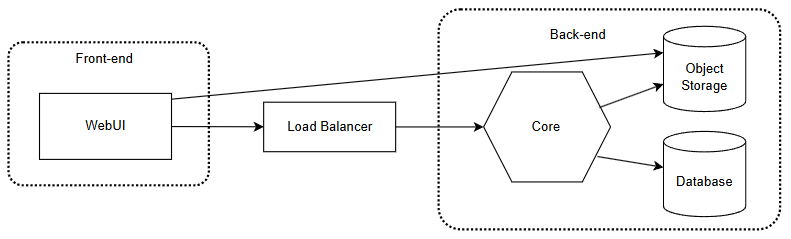
\includegraphics[width=\textwidth]{assets/diagrams/high-level-arch.png}
    \caption{L'architettura di alto livello}
    \label{fig:Architettura di alto livello}
\end{figure}

\begin{figure}[H]
    \centering
    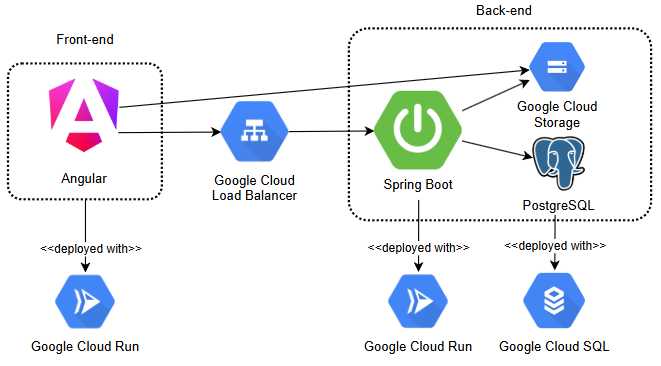
\includegraphics[width=\textwidth]{assets/diagrams/high-level-arch-tecnologies.png}
    \caption{L'architettura di alto livello, con tecnologie}
    \label{fig:Architettura di alto livello, con tecnologie}
\end{figure}

L'infrastruttura scelta per il deployment é Google Cloud, che garantisce availability 
di 99.95\% per i servizi di Run, SQL, Storage, per cui garantisce anche una durability 
ad undici 9.

Angular é stato scelto per implementare il front-end con una SPA (Single Page 
Application). La scelta di un'interfaccia web è figlia dell'obiettivo di alta 
adaptability.

Spring Boot é stato scelto per l'implementazione del core del sistema grazie al ridotto 
time-to-market che esso garantisce e alla sua affidabilitá dovuta al suo massiccio 
utilizzo nell'industria moderna. Spring Boot permette una facile integrazione di un 
potente ORM (Object Relational Mapping) come JPA (Java Persistence API).

PostgreSQL è stato scelto come DBMS per la sua efficienza e per il suo supporto nativo 
ai dati geografici (estensione PostGIS).

La scelta di un unico Cloud Provider permette una riduzione notevole della latenza nelle 
comunicazioni tra i componenti del sistema.

\section{Design del back-end}

\subsection{Persistenza dei dati}
Si presenta adesso lo schema per la persistenza dei dati.
Si é deciso, per alcune tabelle (Listing, User, Notification, Search) di definire
una struttura dotata di ereditarietá, per un'integrazione pulita con lo schema dei dati
del servizio Spring Boot. L'integrazione tra Spring Boot e il database é gestita da JPA.

É fornita ora una brevissima panoramica sulle possibili strategie per
l'implementazione di strutture gerarchiche basate sull'ereditarietá in un
DBMS relazionale.
\subsubsection{Ereditarietá in un DBMS relazionale}
I DBMS relazionali non supportano nativamente l'ereditarietá per come essa é nota
ai conoscitori dei linguaggi object-oriented. Tuttavia, é possibile applicare dei
noti pattern per sopperire a questa limitazione:
\begin{list}{$\cdot$}{}
    \item Single Table: si memorizzano tutti gli attributi di tutte le 
    classi (superclasse e sottoclassi) in un'unica tabella. Include un campo discriminatore 
    che indica il tipo specifico di ogni record.
    \item Joined Table: si crea crea una tabella separata per ogni classe nella gerarchia. 
    La tabella della sottoclasse contiene solo gli attributi specifici e una chiave esterna 
    che punta alla tabella della superclasse.
    \item Table Per Class: si crea una tabella separata e completa per ogni sottoclasse, 
    includendo sia gli attributi ereditati dalla superclasse che quelli specifici.
\end{list}

\begin{table}[H]
    \centering
    \begin{tabularx}{\textwidth}{|X|X|X|X|}
    \hline
    \textbf{Aspetto} & \textbf{Single Table} & \textbf{Joined Table} & \textbf{Table Per Class} \\
    \hline
    \textbf{Spreco di dati} & 
    Alto. Tutti gli attributi di tutte le sottoclassi sono memorizzati in un'unica tabella, con molti valori NULL per gli attributi non pertinenti alla classe specifica. & 
    Basso. Ogni tabella contiene solo gli attributi specifici della classe corrispondente, minimizzando lo spazio inutilizzato. & 
    Medio. Ciascuna tabella è completa ma si ha duplicazione degli attributi della superclasse in ogni tabella delle sottoclassi. \\
    \hline
    \textbf{Velocità di lettura} & 
    Alta. Nessun JOIN necessario per recuperare un oggetto completo, le query sono generalmente più veloci. & 
    Media/Bassa. Richiede JOIN tra le tabelle della gerarchia per ricostruire oggetti completi, penalizzando le performance con gerarchie profonde. & 
    Alta per singole sottoclassi. Bassa per query polimorfiche sulla superclasse che richiedono UNION di tutte le tabelle delle sottoclassi. \\
    \hline
    \textbf{Velocità di inserimento} & 
    Alta. Un singolo INSERT in un'unica tabella. & 
    Media. Richiede INSERT multipli (uno nella tabella della superclasse e uno nella tabella della sottoclasse). & 
    Alta. Un singolo INSERT in una tabella concreta. \\
    \hline
    \textbf{Velocità di aggiornamento} & 
    Alta. UPDATE su un'unica tabella. & 
    Media. Può richiedere UPDATE su più tabelle se si modificano attributi ereditati. & 
    Alta per attributi specifici, ma richiede aggiornamenti multipli se si modificano gli stessi attributi in classi differenti. \\
    \hline
    \end{tabularx}
    \caption{Confronto tra strategie di implementazione dell'ereditarietà in JPA}
    \label{tab:inheritance-comparison}
    \end{table}

Alla luce di questa disamina, si é deciso di:
\begin{list}{$\cdot$}{}
    \item applicare la strategia Joined Table per la gerarchia con radice la tabella USER, in quanto
    is prevede che il numero di utenti di tipo CUSTOMER sia maggiore 
    degli altri di diversi ordini di grandezza.
    \item applicare la strategia Single Table per le gerarchie di SEARCH,
    LISTING: HOUSE é, secondo le stime, la sottoclasse che
    avrá piú istanze, di gran lunga sulle altre.
    \item applicare la strategia Single Table per la gerarchia di NOTIFICATION:
    i campi nulli sono pochi. Inoltre, la tabella NOTIFICATION é una mera tabella
    di outbox (si parlerá di seguito dell'outbox pattern), per cui le sue righe sono
    destinate ad essere eliminate in tempi brevi.
\end{list}

Si motiva adesso l'esistenza della tabella NOTIFICATION.
\subsubsection{L'OUTBOX Pattern}
Il pattern Outbox rappresenta una soluzione elegante al problema della comunicazione affidabile 
tra servizi distribuiti, specialmente in contesti in cui la coerenza dei dati é fondamentale.
Nel nostro caso, non parliamo di coerenza di dati, ma semplicemente di affidabilitá di comunicazione:
una notifica persa é potenzialmente un grave problema nell'esperienza degli utenti: si pensi al caso 
in cui un agente accetti una richiesta di visita, ma la notifica non arrivi al cliente.

L'idea alla base è semplice: sfruttare le proprietá ACID di un DBMS (tipicamente relazionale) per 
inserire un evento e la comunicazione di esso all'interno della stessa transazione, inserendo la 
comunicazione in una tabella di OUTBOX.
Nel nostro caso, la tabella NOTIFICATION é una tabella di OUTBOX, da cui poi il sistema
potrá attingere per inviare le comunicazioni. Una volta consumate, le comunicazioni sono
rimosse dalla tabella.

\begin{figure}[H]
    \centering
    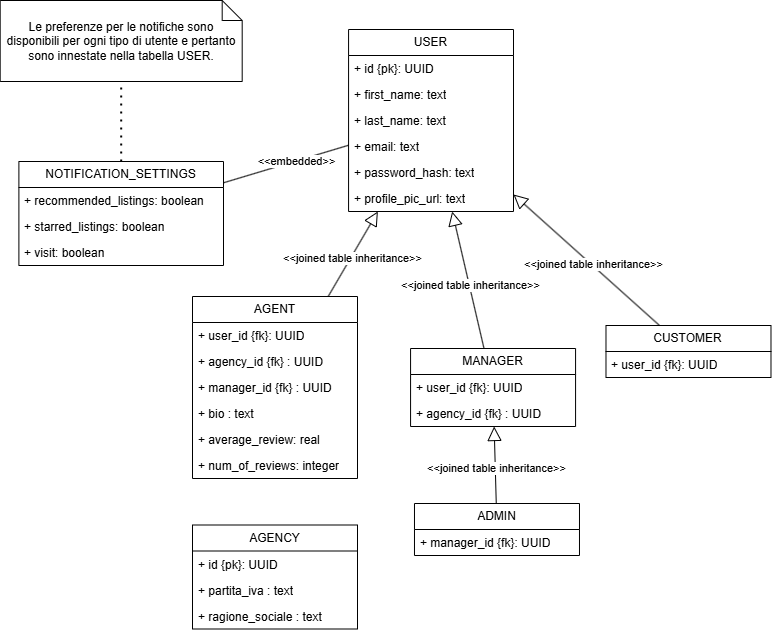
\includegraphics[width=\textwidth]{assets/diagrams/db-scheme/users.png}
    \caption{Lo schema di persistenza degli utenti.}
    \label{fig:Schema di persistenza degli utenti}
\end{figure}

\begin{figure}[H]
    \centering
    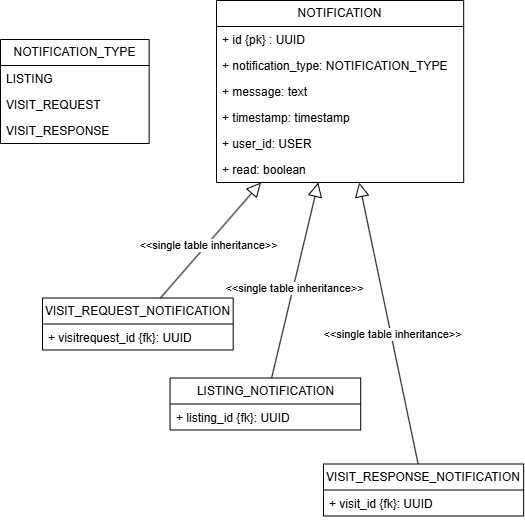
\includegraphics[width=\textwidth]{assets/diagrams/db-scheme/notification.png}
    \caption{Lo schema di persistenza delle notifiche.}
    \label{fig:Schema di persistenza delle notifiche}
\end{figure}

\begin{figure}[H]
    \centering
    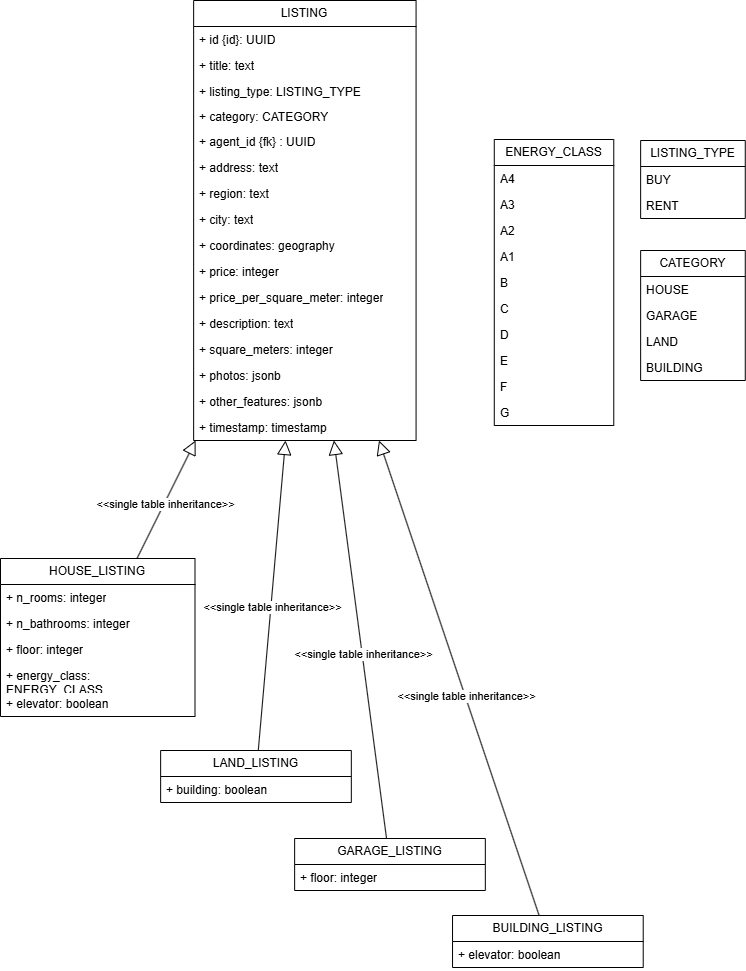
\includegraphics[width=\textwidth]{assets/diagrams/db-scheme/listing.png}
    \caption{Lo schema di persistenza degli annunci.}
    \label{fig:Schema di persistenza degli annunci}
\end{figure}

\begin{figure}[H]
    \centering
    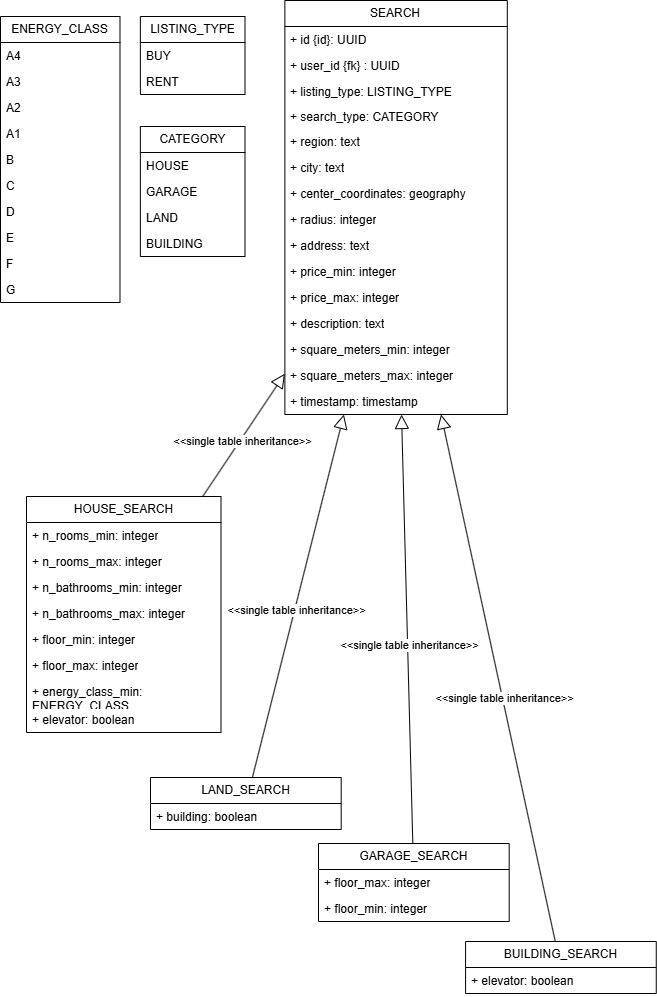
\includegraphics[width=\textwidth]{assets/diagrams/db-scheme/search.png}
    \caption{Lo schema di persistenza delle ricerche effettuate dagli utenti.}
    \label{fig:Schema di persistenza delle ricerche effettuate dagli utenti}
\end{figure}

\subsection{L'architettura esagonale}
La scelta di un framework opinionated come Spring Boot impone un’architettura ben precisa: 
l'architettura esagonale, anche detta port-and-adapters, formalizzata da A. Cockburn.

L’obiettivo di questa architettura é rendere il cosiddetto core facilmente testabile, 
manutenibile e molto agile di fronte a cambiamenti ed estensioni, permettendo di non 
stravolgere la codebase.

Per ottenere ciò, l’architettura esagonale definisce un confine netto tra il core e 
le estensioni, chiamate porte, che definiscono un contratto tra il core ed il componente 
esterno che fornisce l’estensione. Tale componente esterno é chiamato adapter.
Bisogna fare un distinguo tra porte in entrata e porte in uscita:
\begin{list}{$\cdot$}{}
    \item porte in entrata, spesso chiamate Service come nel caso di Spring, sono spesso 
    mappate a use case e definiscono possibili microservizi.
    \item porte in uscita sono interfacce che definiscono come il core puó utilizzare 
    un componente esterno.
\end{list}

Tale distinguo si riflette sugli adapter:
\begin{list}{$\cdot$}{}
    \item adapter in entrata, spesso chiamati Controller come nel caso di Spring, 
    usano le porte in entrata.
    \item adapter in uscita implementano le porte in uscita.
\end{list}

Sia le porte che gli adapter per la persistenza dei dati sono spesso chiamate Repository, 
come nel caso di Spring.

\begin{figure}[H]
    \centering
    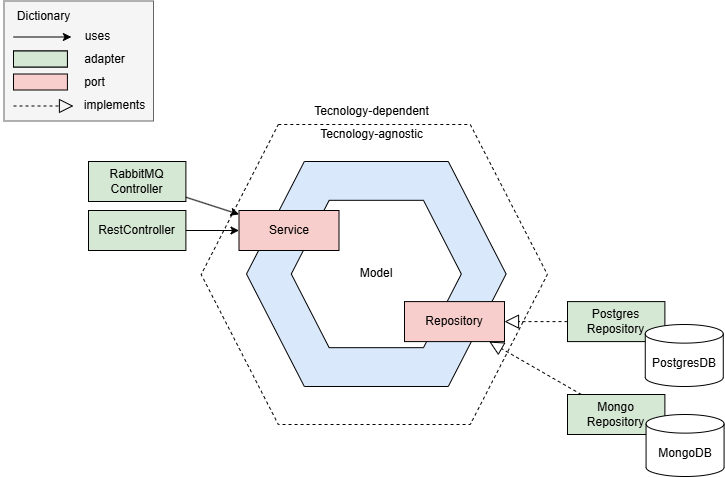
\includegraphics[width=\textwidth]{assets/diagrams/hexagonal-architecture.png}
    \caption{Un esempio di architettura esagonale.}
    \label{fig:un esempio di architettura esagonale}
\end{figure}

L’architettura esagonale: 
\begin{list}{$\cdot$}{}
    \item permette un testing efficace del core grazie alla dependency injection 
    alla base: il mocking delle dipendenze è molto semplificato.
    \item facilita l’aggiunta di nuove feature: si definisce una porta e la si 
    adatta con una tecnologia specifica.
    \item permette una migrazione naturale ad architetture piú modulari dal punto 
    di vista del deployment, come modular monolith e microservizi.
\end{list}

\subsection{Diagramma dei package}
Vengono presentati adesso i package che compongono il software.
\begin{list}{$\cdot$}{}
    \item auth: al suo interno é definita la logica di autenticazione del sistema ed
    e le operazioni su generici utenti. Viene impiegato al suo interno Spring Security,
    il modulo di Spring per la gestione della sicurezza.
    \item customer: al suo interno é definita la logica per la gestione
    dei clienti.
    \item agency: al suo interno é definita la logica per la gestione
    dell'agenzia e delle figure che la compongono: amministratore, gestori, agenti.
    \item listing: contiene la logica di creazione, gestione, ricerca di annunci.
    \item visit: contiene la logica per quanto concerne le richieste di visita e 
    le visite.
    \item agentreview: al suo interno vi é la logica di creazione e visualizzazione di 
    valutazioni degli agenti.
    \item starredlisting: contiene la logica della funzionalitá secondo cui
    un utente puó inserire tra i preferiti un annuncio.
    \item notification: definisce la logica di creazione ed invio delle
    notifiche.
\end{list}

\begin{figure}[H]
    \centering
    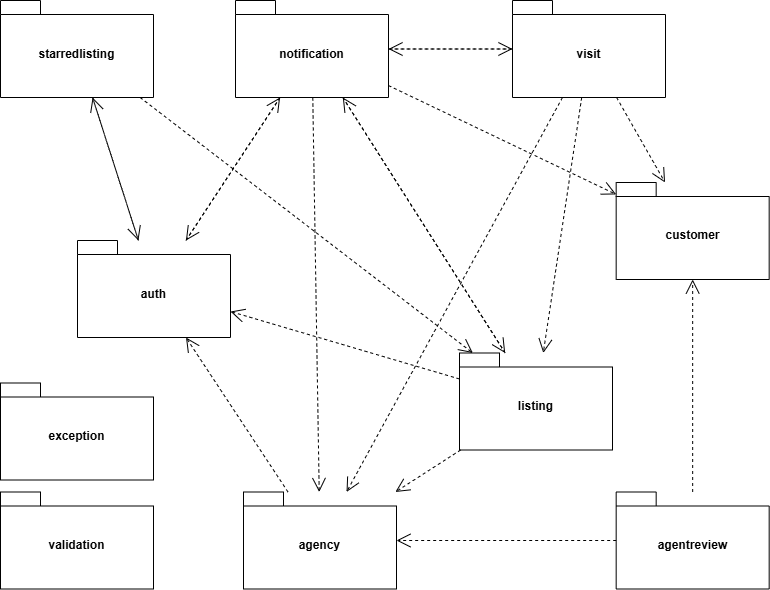
\includegraphics[width=\textwidth]{assets/diagrams/class-diagram/package.png}
    \caption{Il diagramma dei package.}
    \label{fig:Diagramma dei package}
\end{figure}

\begin{figure}[H]
    \centering
    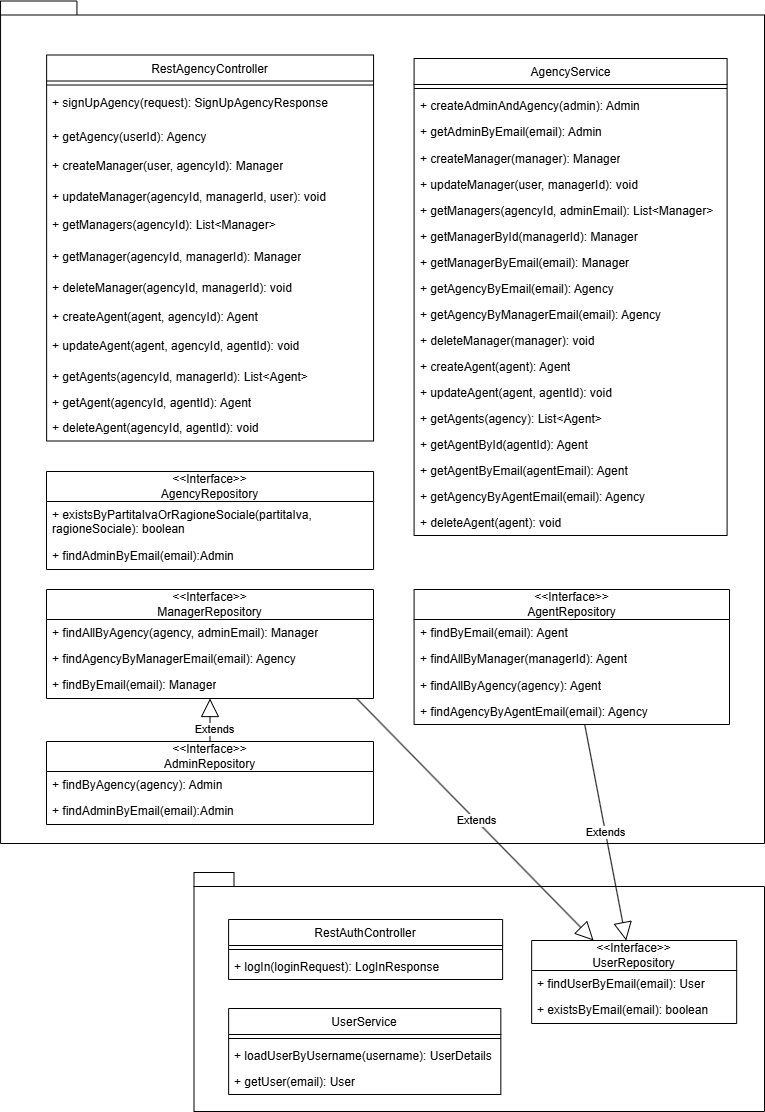
\includegraphics[width=\textwidth]{assets/diagrams/class-diagram/class-diagram-1.png}
    \caption{Parte del diagramma delle classi.}
    \label{fig:Parte 1 del diagramma delle classi}
\end{figure}

\begin{figure}[H]
    \centering
    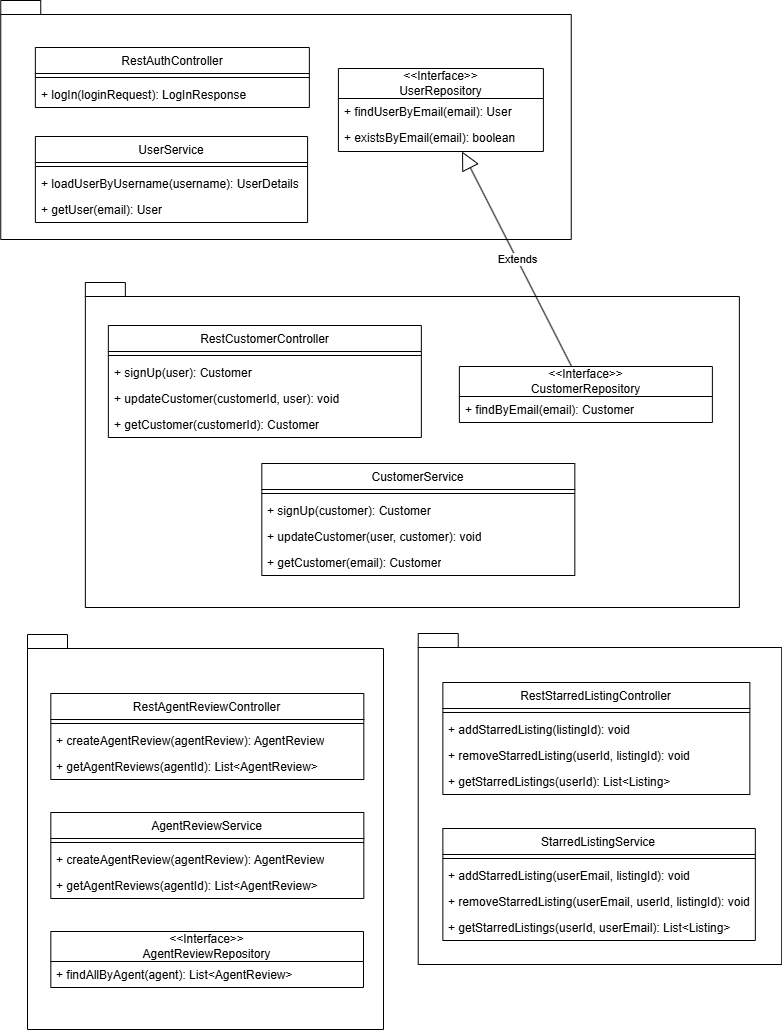
\includegraphics[width=\textwidth]{assets/diagrams/class-diagram/class-diagram-2.png}
    \caption{Parte del diagramma delle classi.}
    \label{fig:Parte 2 del diagramma delle classi}
\end{figure}

\begin{figure}[H]
    \centering
    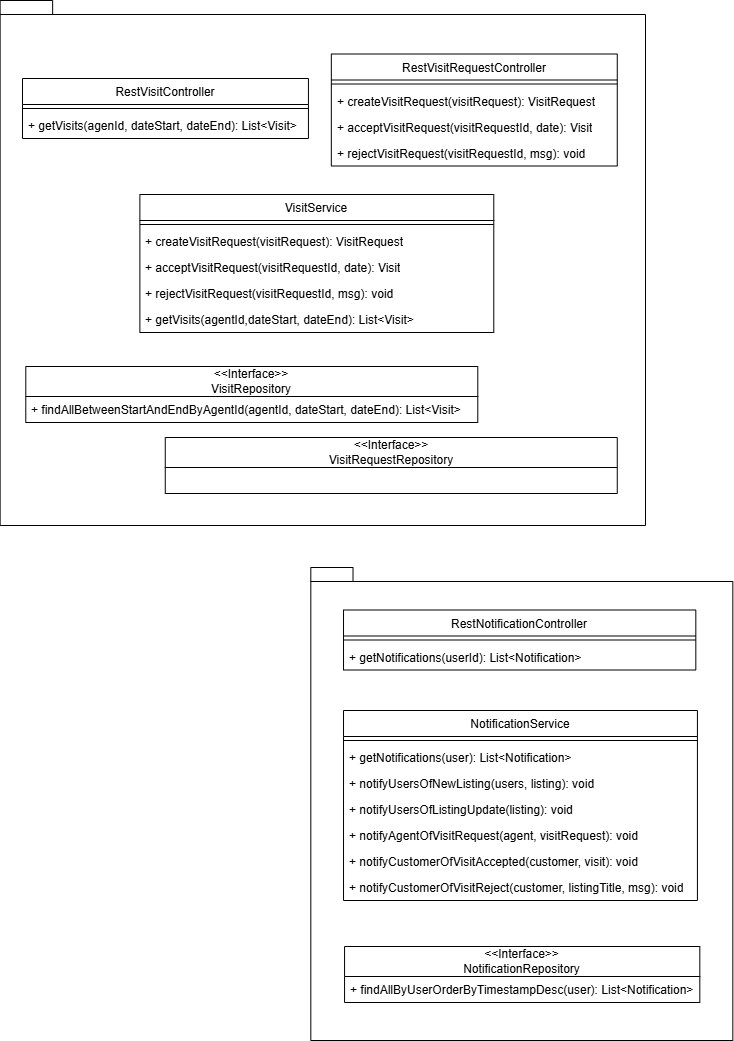
\includegraphics[width=\textwidth]{assets/diagrams/class-diagram/class-diagram-3.png}
    \caption{Parte del diagramma delle classi.}
    \label{fig:Parte 3 del diagramma delle classi}
\end{figure}

\begin{figure}[H]
    \centering
    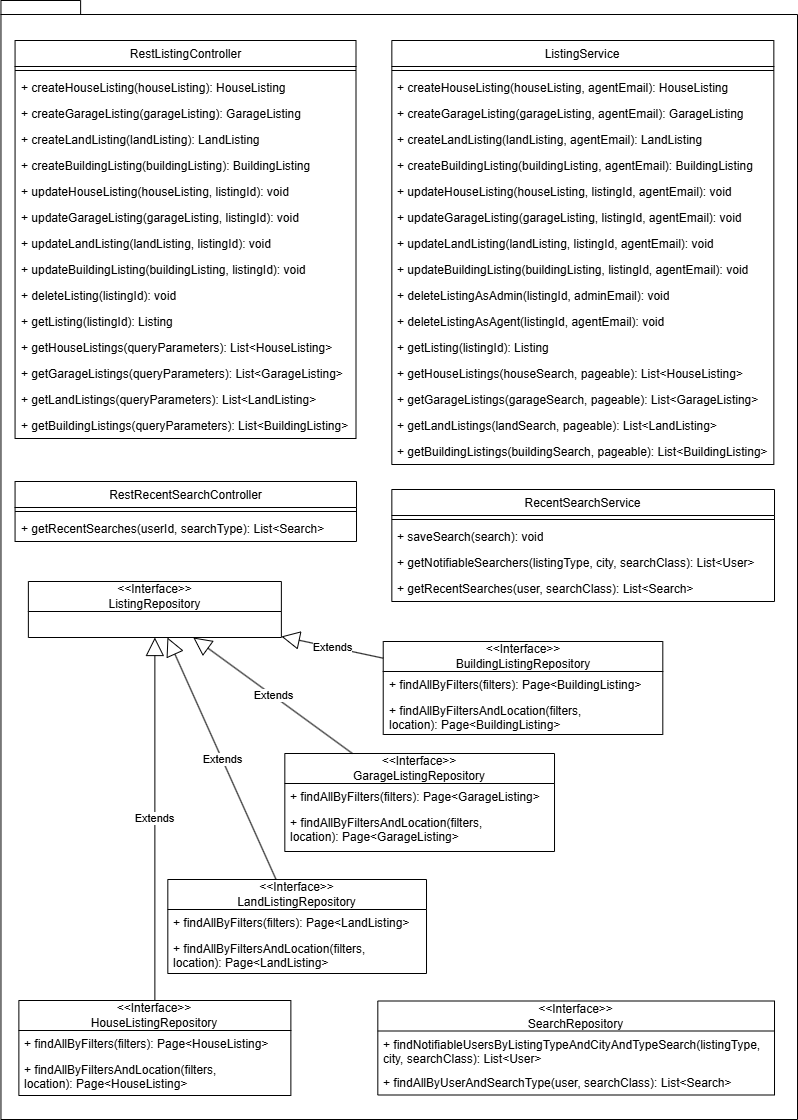
\includegraphics[width=\textwidth]{assets/diagrams/class-diagram/class-diagram-4.png}
    \caption{Parte del diagramma delle classi.}
    \label{fig:Parte 4 del diagramma delle classi}
\end{figure}

\subsection{Diagrammi di sequenza}
Vengono adesso documentati alcuni casi d'uso tramite diagramma di sequenza.

\begin{figure}[H]
    \adjustbox{width=1.4\textwidth,center}{
        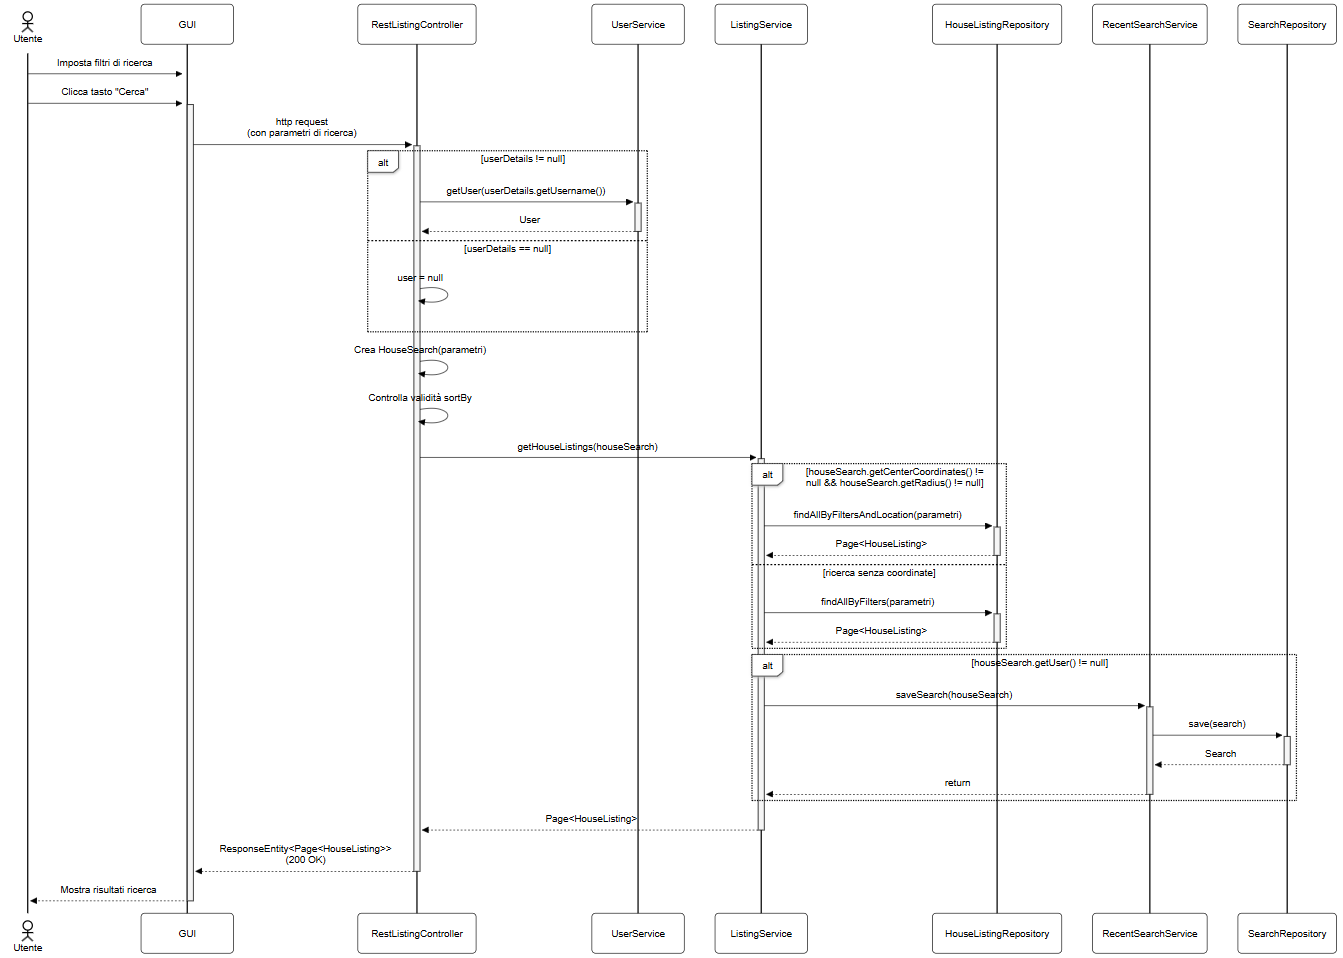
\includegraphics{assets/diagrams/sequence/ricerca-immobili.png}
    }
    \caption{Diagramma di sequenza del caso d'uso Ricerca Immobili.}
    \label{fig:Diagramma di sequenza del caso d'uso Ricerca Immobili}
\end{figure}

\begin{figure}[H]
    \adjustbox{width=1.4\textwidth,center}{
        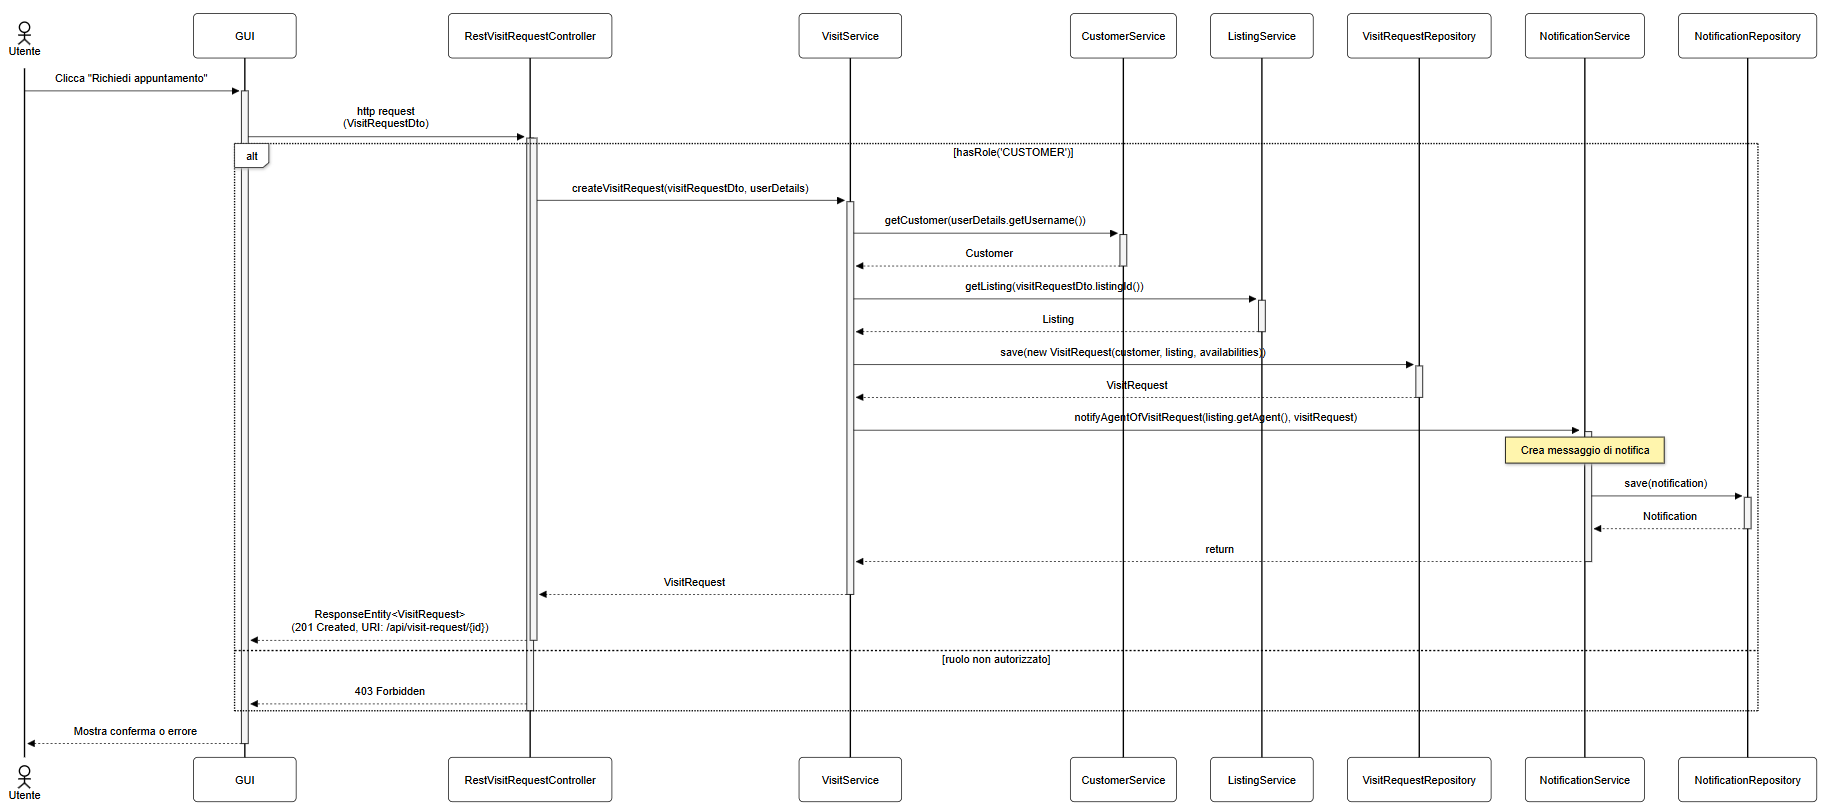
\includegraphics[width=\textwidth]{assets/diagrams/sequence/fissa-appuntamento.png}
    }
        \caption{Diagramma di sequenza del caso d'uso Fissa Appuntamento.}
    \label{fig:Diagramma di sequenza del caso d'uso Fissa Appuntamento}
\end{figure}

\begin{figure}[H]
    \adjustbox{width=1.4\textwidth,center}{
        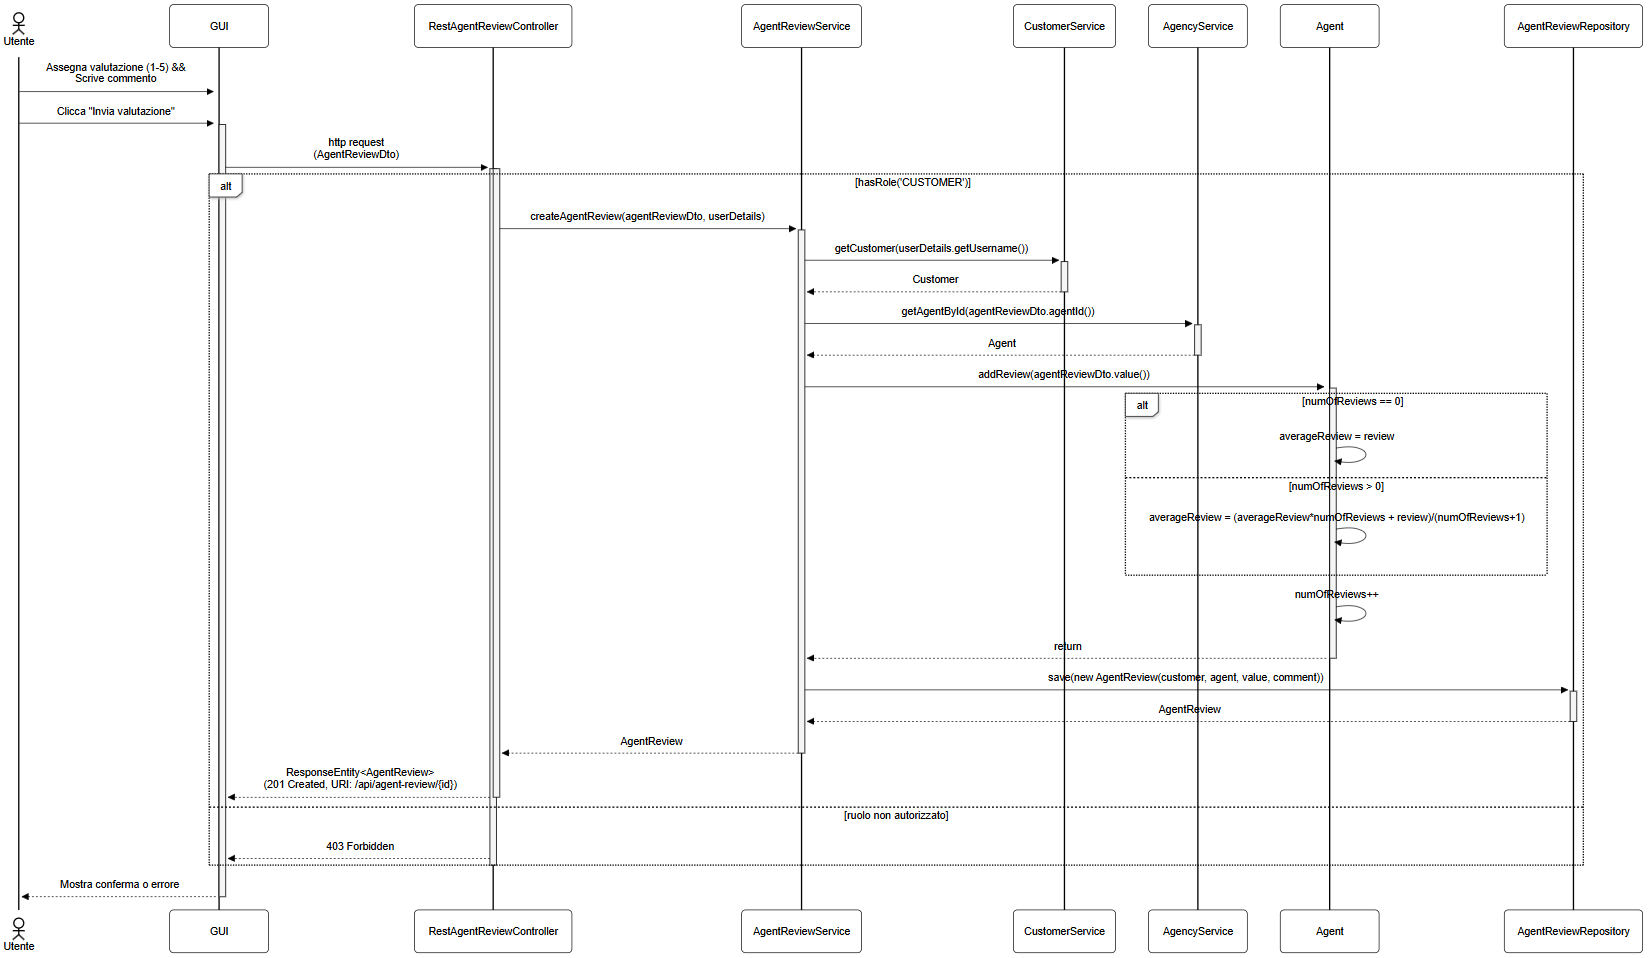
\includegraphics[width=\textwidth]{assets/diagrams/sequence/valuta-agente.png}
    }
        \caption{Diagramma di sequenza del caso d'uso Valuta Agente.}
    \label{fig:Diagramma di sequenza del caso d'uso Valuta Agente}
\end{figure}

\begin{figure}[H]
    \adjustbox{width=1.4\textwidth,center}{
        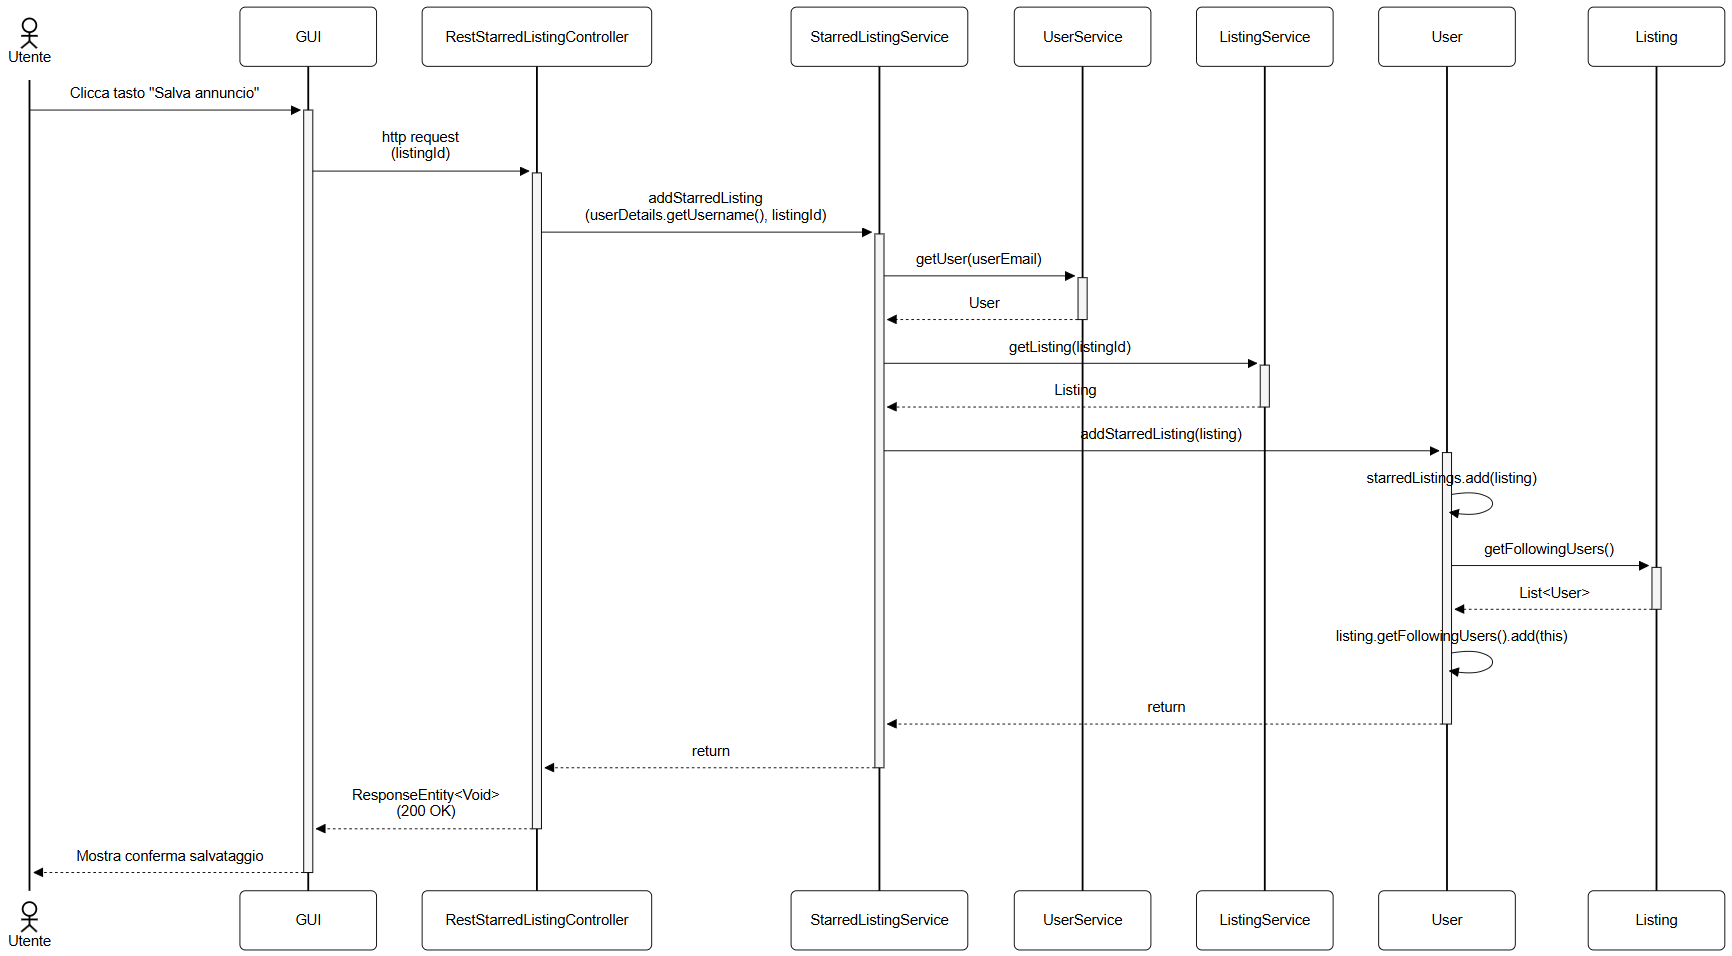
\includegraphics[width=\textwidth]{assets/diagrams/sequence/salva-annuncio.png}
    }
    \caption{Diagramma di sequenza del caso d'uso Salva Annuncio.}
    \label{fig:Diagramma di sequenza del caso d'uso Salva Annuncio}
\end{figure}

\section{Design dell'interfaccia utente}
L'interfaccia utente deve rispettare le 10 regole euristiche per l'usabilitá
di Nielsen e Molich:
\begin{enumerate}
    \item Simple and Natural Dialogue: l'interfaccia deve essere semplice e minimale, in modo da rendere l'esperienza
    intuitiva e priva di superflue distrazioni.
    \item Speak the User's Language: l'interfaccia deve usare parole, frasi e concetti familiari all'utente, 
    evitando tecnicismi o termini da sviluppatori.
    \item Minimize User Memory Load: gli utenti non dovrebbero dover ricordare informazioni da una parte 
    dell'interfaccia all'altra. I dati e le istruzioni devono essere visibili 
    o facilmente recuperabili.
    \item Consistency: l'interfaccia deve essere coerente nell'uso di colori, termini, pulsanti e layout. 
    Le stesse azioni devono produrre risultati simili.
    \item Feedback: il sistema deve fornire all'utente un riscontro immediato e comprensibile 
    per ogni azione eseguita.
    \item Clearly Marked Exits: gli utenti devono poter annullare azioni o uscire da situazioni senza sentirsi bloccati.
    \item Shortcuts: gli utenti esperti devono poter usare scorciatoie da tastiera, menu rapidi o comandi 
    per lavorare più velocemente.
    \item Good error messages: i messaggi d'errore devono essere chiari, indicare il problema e suggerire come risolverlo.
    \item Prevent Errors: l'interfaccia deve essere progettata per prevenire gli errori prima che avvengano, tramite controlli e vincoli.
    \item Help and Documentation: anche se l'interfaccia dovrebbe essere intuitiva, è utile offrire supporto accessibile e facilmente comprensibile 
    per risolvere problemi o approfondire funzionalità.
\end{enumerate}